\documentclass[titlepage]{article}
\usepackage[parfill]{parskip}
\usepackage[utf8]{inputenc}
\usepackage{float}
\usepackage{graphicx}
\graphicspath{ {./graphs/} }

\title{Computer Science 2XC3 Lab 4/5}
\author{Gregory Archer, Will Clubine, Gaurav Sharma}
\date{February 8th 2023}

\begin{document}

\maketitle
\tableofcontents
\listoffigures

\newpage

\section{Executive Summary}
\begin{itemize}
    \item Experiment 1 showed that
    \item Experiment 2 showed that
\end{itemize}

\section{Part 1}

\subsection{Experiment 1}

Experiment 1 examines the probability of a graph containing cycles as the proportion of edges to nodes increases.

The probability of a graph containing a cycle was computed by generating 500 random graphs with a given number of edges and nodes, and observing how many were cyclical.

We completed this process for graphs containing 5, 10, 15 and 20 nodes, with the proportion of edges varying from 0\% to 120\%, in increments of 20\%.

The result was then graphed in Figure 1 below.

\begin{figure}[H]
    \centering
    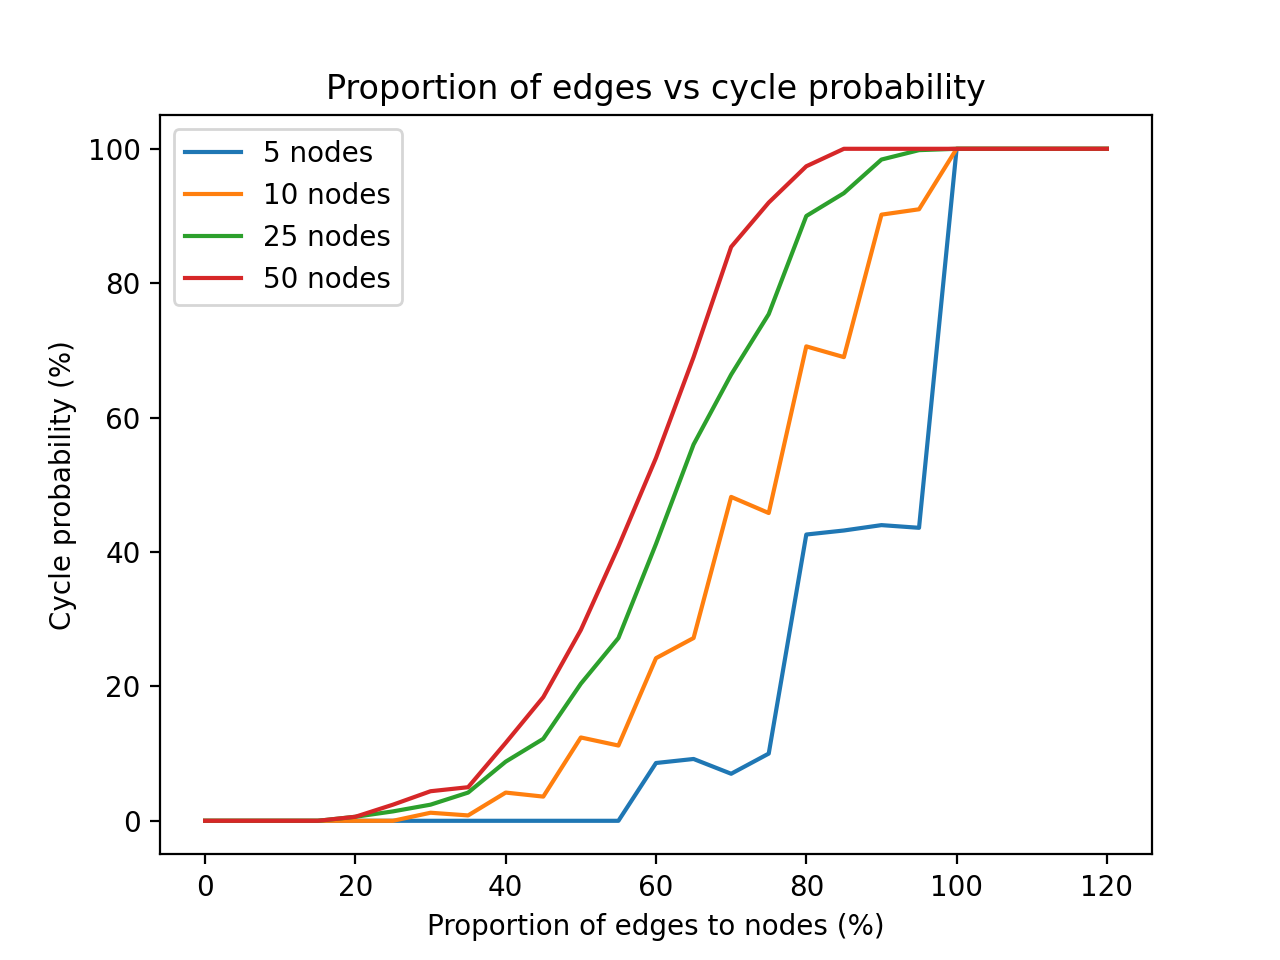
\includegraphics[width=0.8\linewidth]{experiment_1.png}
    \caption{Proportion of edges vs cycle probability}
    \label{fig:edges_vs_cycle}
\end{figure}

We have concluded from our results that as the proportion of edges relative to the number of nodes increases, the cyclical probability grows, showing a direct correlation. As the number of nodes increases, the probability of a graph containing a cycle - with the same relative proportions - increases, showing another direct correlation

Additionally, once the proportion of edges to nodes is 100\%, there will always be a cycle in the graph, regardless of the number of nodes. This is expected as any graph with equal or more edges than nodes must contain a cycle.

\subsection{Experiment 2}

Experiment 2 examines the probability of a graph being connected as the proportion of edges to nodes increases.

We compute the approximate connected probability for a graph of $e$ edges and $n$ nodes by generating 500 random graphs with $e$ edges and $n$ nodes and determining what percentage of those graphs are connected.

This process is conducted for graphs with 5, 10, 25, and 50 nodes at different proportions of edges. Specifically, we start with 0 edges and gradually increase to 500\% the node count in 20\% increments. The result is then graphed as shown in Figure \ref{fig:edges_vs_connected} below.

\begin{figure}[H]
    \centering
    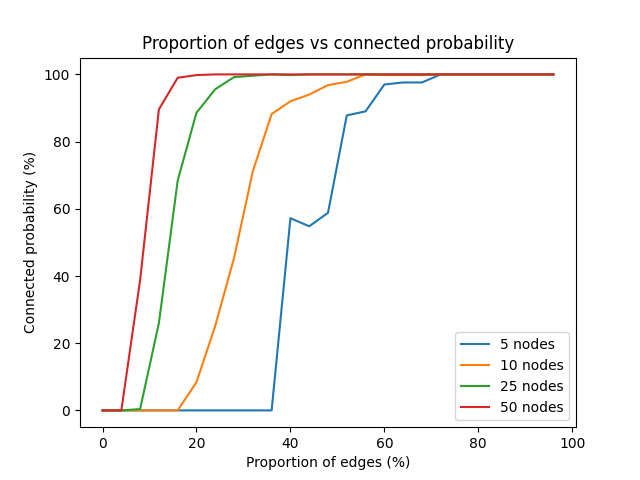
\includegraphics[width=0.8\linewidth]{experiment_2.png}
    \caption{Proportion of edges vs connected probability}
    \label{fig:edges_vs_connected}
\end{figure}

% this is wrong v will rewrite

As seen in Figure \ref{fig:edges_vs_connected}, each graph sits at a 0\% chance of connectedness before rapidly increasing and eventually reaching a 100\% probability of being connected. However, the proportion of edges at which the probability starts and stops rising increases with the number of nodes.

This is because the maximum number of unique edges --- and thus the number of ways the graph can be disconnected --- grows quadratically with the number of nodes. Specifically, a graph of $n$ nodes with no self-loops can have a maximum of $\Sigma_{i=0}^{n-1}i = \frac{(n - 1) \cdot n}{2}$ unique edges. This means a graph of 5 nodes has already reached it's maximum number of edges (10) by 200\%, while a graph of 50 nodes will not reach it's maximum number of edges (1225) until 2450\%.

\section{Part 2}

\subsection{Minimum Vertex Cover Approximation}
Throughout all of the minimum vertex cover experiments, the accuracy of all approximation algorithms will be compared to the result of the minimum vertex cover algorithm provided. 

\subsubsection{Experiment 1}
In the first experiment, we determined how each approximation algorithm's expected performance differs as the number of edges in a graph increases. Each algorithm was tested against 28 cases. The number of nodes between test cases was constant and the number of edges varied. The first case consisted of a graph with 8 nodes and 1 edge, every subsequent case increased the number of edges by 1, resulting in a final case of 8 nodes and 28 edges. Notably, the final case has the maximum number of unique edges for an undirected graph of 8 nodes.

An approximation algorithm's expected performance was calculated by summing the output 1000 times for each test case and dividing it by the sum of the actual number of nodes in the minimum vertex cover. In mathematical notation, the expected performance of $approx1()$ was calculated by:
\[ \sum_{n=1}^{1000} approx1(G_n) \quad \div \quad \sum_{n=1}^{1000} MVC(G_n)\]
where $G_i$ represents the $ith$ random graph for a given test case.

The larger the expected performance, the further it was from the minimum vertex cover. For example, a value of 2 would mean that the algorithm's average output would be twice as long as the list of nodes in the minimum vertex cover. The lowest and best performance would be a value of 1, as this means the average approximate is the same length as the minimum vertex cover.

\begin{figure}[H]
    \centering
    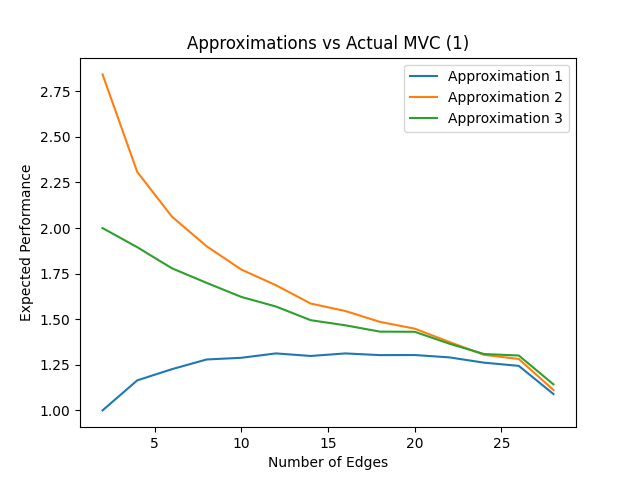
\includegraphics[width=0.8\linewidth]{experiment_3_1.png}
    \caption{The Expected Performance of Approximation Algorithms as Edges Increase}
    \label{fig:experiment_3_1}
\end{figure}

As seen from Figure \ref{fig:experiment_3_1}, every approximation algorithm converged to an expected performance value of roughly 1.1. This makes sense, as the number of edges in a graph approaches the maximum number of unique edges, the number of nodes in the minimum vertex cover will converge to a value. In the case of 8 nodes, the minimum vertex cover will always be 7 nodes. Since it is impossible to output more nodes than there are present in the graph, the approximation algorithms can only return 7 or 8 nodes. As the length of the minimum vertex cover grows, the chance that an algorithm overestimates the number of nodes in the minimum vertex cover drastically decreases. Thus the accuracy of the approximations will be far greater than graphs with fewer edges. This is extremely apparent in a comparison of the expected performance between graphs with 27 edges and 28 edges. All approximation algorithms perform significantly better when the number of edges is the maximum number of unique edges possible.

The first approximation algorithm, $approx1()$ performed the best in this experiment, as its average output was more accurate than the other algorithms for all test cases. However, unlike the other algorithms, $approx1()$ performed worse as edges increased. For the first two test cases, the algorithm achieved a perfect value of 1, but as the number of edges increased, the expected performance worsened, until around 21 edges when the performance improved again. Since this algorithm chooses nodes based on their degree, it makes sense that it performs well for graphs with few edges. The algorithm will hone in on the few nodes with edges, meaning it will always choose the minimum number of nodes. As the number of edges increases, it is more likely for the algorithm to erroneously add nodes that are not part of the minimum vertex cover as there are simply more edges present in the graph. Finally, as the number of edges approaches the maximum number of edges, the chance that a node is added which isn't in the minimum vertex cover drastically decreases. 

The second approximation algorithm, $approx2()$ performed the worst in this experiment, as its average output was far less accurate than the other algorithms until the last test cases.
The randomness of $approx2()$ is the main contributing factor to why its performance is so terrible. At its worst, the algorithm is expected to return an output that is three times the size of the minimum vertex cover! Since the algorithm has no intelligent way of selecting a node, for graphs with few edges, it is likely for the chosen node to be completely unconnected. Such unconnected edges contribute nothing to the vertex cover. As the number of edges increases, the chance of the algorithm choosing an unconnected node decreases, thus the performance of this algorithm improves.

The third approximation algorithm, $approx3()$ fared better than $approx2()$ for the majority of the test cases until the very end. Similar to the second approximation algorithm, this algorithm relies on randomness and will likely add nodes that shouldn't be in the minimum vertex cover. However, since the algorithm is randomly selecting edges rather than nodes, it will never include unconnected nodes. Interestingly, this algorithm returns twice the number of nodes for the first 2 test cases. This is because a major downfall of this algorithm is that it can only return nodes in multiples of 2. For a graph with a minimum vertex cover with 1 node, this algorithm will always return 2 nodes. This is why this algorithm begins to perform worse than $approx2()$ for the last couple of test cases. In cases where the minimum vertex cover is 7 nodes, $approx2()$ will likely output 7 nodes, whereas $approx3()$ will always output 8 nodes.


Overall, the first experiment shows that approximation algorithms will converge as edges approach the maximum number of unique edges in an undirected graph. Additionally, although all algorithms perform relatively accurately when given a graph with the maximum number of edges, $approx1()$ performs far better for most test cases, especially for graphs with few edges.

\subsubsection{Experiment 2}

In the second experiment, we determined how each approximation algorithm's expected performance differs as the number of nodes in a graph increases. Each algorithm was tested against 12 cases. The number of nodes between test cases varied and the number of edges was constant. The first case consisted of a graph with 4 nodes and 6 edges, every subsequent case increased the number of nodes by 1, resulting in a final case of 11 nodes and 6 edges. Notably, the first case has the maximum number of unique edges for an undirected graph of 4 nodes.

An approximation algorithm's expected performance was calculated in the same way as Experiment 1. The sum of the lengths of approximated vertex covers was divided by the sum of the lengths of minimum vertex covers. The larger the expected performance, the further it was from the minimum vertex cover.

\begin{figure}[H]
    \centering
    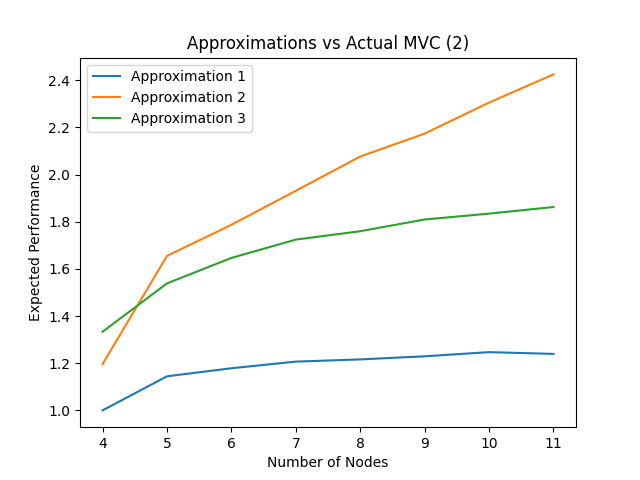
\includegraphics[width=0.8\linewidth]{experiment_3_2.png}
    \caption{The Expected Performance of Approximation Algorithms as Nodes Increase}
    \label{fig:experiment_3_2}
\end{figure}

As seen from Figure \ref{fig:experiment_3_2}, the approximations seem to diverge, a far cry from experiment 1, where they converged. Each algorithm saw a major hit (relative to the rest of their growth) in expected performance in the jump from 4 nodes to 5 nodes. This follows from the observations in Experiment 1, where all the approximations algorithms performed far better on graphs with the maximum number of unique edges.

The first approximation algorithm, $approx1()$ performed the best in this experiment, as its average output was more accurate than the other algorithms and the expected performance stayed consistent as nodes grew. Since the number of edges remained constant, the additional nodes added are likely to be unconnected. As established in Experiment 1, this algorithm ignores unconnected nodes and thus is independent of the number of nodes in a graph.

The second approximation algorithm, $approx2()$ performed the worst for the majority of this experiment. This follows from experiment 1, since this algorithm randomly selects nodes, the more unconnected nodes there are present in the graph, the more likely that this algorithm will randomly select them instead of nodes with edges. Thus, this algorithm will perform far worse as the number of nodes increases.

The third approximation algorithm, $approx3()$ fares better than approximation 2 mainly from it being more selective in its randomness. Since it randomly chooses an edge, it completely avoids choosing unconnected nodes, rather the extra performance comes from the fact that this algorithm can only output nodes in multiples of 2. Meaning, with graphs with few nodes in the minimum vertex cover, it is likely for this algorithm to add extra incident nodes that aren't part of the vertex cover. Hence why the algorithm's expected performance isn't as bad as approximation 2 as nodes grow.

Overall, the second experiment showed that the approximation algorithms differ greatly as nodes increase. Approximation 1 is independent to the number of nodes present in the graph unless the graph's number of edges is the maximum number of edges for that number of nodes. Whereas, approximation 2 depends greatly on the number of nodes. Finally approximation 3 is dependent on the number of nodes but far less than approximation 2.

\subsubsection{Experiment 3}



\subsection{Maximum Independent Sets}

To determine the relationship between minimum vertex covers (MVC) and maximum independent sets (MIS), we compared their average size for graphs of 10 nodes with 0 to 45 edges; the maximum for a graph of 10 nodes. At each number of edges, we found the MVC and MIS for 250 graphs and calculated the average length of each, as well as the sum of the average lengths. The results were then graphed as shown in Figure \ref{fig:mvc_mis} below.

\begin{figure}[H]
    \centering
    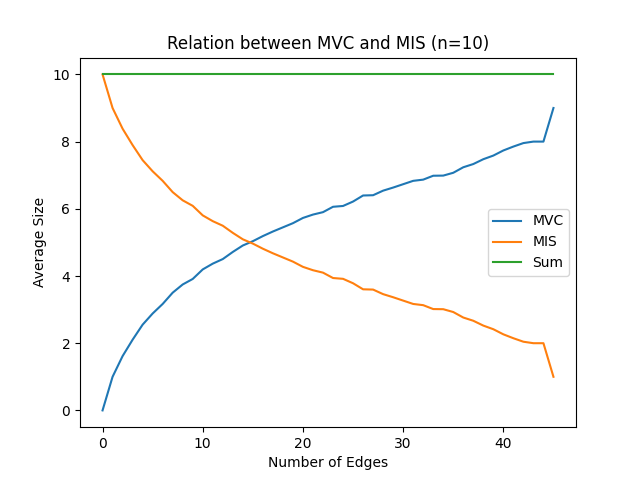
\includegraphics[width=0.8\linewidth]{mvc_mis.png}
    \caption{Relation between MVC and MIS}
    \label{fig:mvc_mis}
\end{figure}

As seen in Figure \ref{fig:mvc_mis}, the average MIS length decreased as the number of edges increased, while the average MVC length increased. Further, their sum was exactly equal to the number of nodes.

Looking closer, we can see that at 0 edges the MVC was empty while the MIS contained all nodes. This is expected because every node can be added to the MIS without connecting to another node, and there are no edge endpoints to be included in the MVC.

At the maximum number of edges, the MIS contains only one node while the MVC contains $n-1$ nodes. This is also expected, because the single node in the MIS connects to all other nodes, and the single node left out of the MVC has every edge taken care of by a node it is connected to.

These three observations leads us to the conclusion that the MVC of a graph is the complement of the MIS.

\appendix
\section{Navigating the Code}

\begin{itemize}
    \item Each experiment in Part 1 can be found within it's own file titled \verb|experiment_#.py|
    \item Approximation experiments can be found within \verb|approximation_experiments.py|
    \item Maximum independent set experiments can be found within \verb|independent_sets.py|
    \item Additional graph functions were added to \verb|graph.py|
\end{itemize}

\end{document}
